\documentclass[beamer]{standalone}
\begin{document}

\title[Electronics] % (optional, use only with long paper titles)
{
	Full network analysis.
}


\begin{frame} 
\titlepage
\end{frame}

\begin{frame}
\frametitle{Outline}
\tableofcontents
% You might wish to add the option [pausesections]
\end{frame}

\section{Some More Organizational Comments}
\begin{frame}
\frametitle{Comments on Lab Books}
\begin{block}{Type of lab book}
 \begin{itemize}
  \item No spiral-bound notebooks, only `real' bound lab books.
  \item Write in pen.
  \item These are \textbf{requirements} for the future labs (\textit{i.e.} you may need a different lab book).
 \end{itemize}
\end{block}
\end{frame}

\begin{frame}
\frametitle{Comments on Lab Books}
\begin{block}{Structure}
 \begin{itemize}
  \item Lab book should stand on its own, it should not require the lab manual to understand what is going on.
  \item Each week there should be an introduction, short explanation for each part of the lab.
  \item Data analysis and answers to questions in the lab manual should be in the main section.  Leave space to paste tables or graphs in the appropriate section.
  \item Conclusion should go through the important data and the important concepts learned (couple of paragraphs).  No new data or results in the conclusion.
 \end{itemize}
\end{block}
\end{frame}

\begin{frame}
\frametitle{Comments on Lab Books}
\begin{block}{Diagrams}
 \begin{itemize}
  \item Diagrams should be labeled: what is shown, which resistors are being used?
  \item Indicate where you connected the ammeter, voltmeter, ohmmeter, etc.
 \end{itemize}
\end{block}
\begin{block}{Grading of lab book}
 \begin{itemize}
  \item For first lab book: very lenient grading.
  \item Where the grader commented, you will get points subtracted next time.
 \end{itemize}
\end{block}
\end{frame}

\begin{frame}
\frametitle{Uncertainties on Measurements}
\begin{block}{Measurements}
 \begin{itemize}
  \item Measurements should be state with an uncertainty.
  \item Uncertainties don't need to be 100\% correct, but should be reasonable.
 \end{itemize}
\end{block}
\begin{block}{Error Propagation}
 \begin{itemize}
  \item No exact error propagation required; using percent error and significant digits is enough.
  \item Do not write 16 significant figures just because your calculator has a screen that long.
 \end{itemize}
\end{block}
\end{frame}

\begin{frame}
\frametitle{Data and Graphs}
\begin{block}{Raw data}
 \begin{itemize}
  \item Record raw data immediately into your lab book so it will never be lost.
  \item If appropriate, \textbf{in addition} record it into a spreadsheet for processing.
 \end{itemize}
\end{block}
\begin{block}{Graphs and trendlines}
 \begin{itemize}
  \item Graphs should have clearly visible data points and error bars.
  \item Do not connect data points with meaningless lines, but draw a trendline or fitted curve if appropriate.
 \end{itemize}
\end{block}
\end{frame}

\section{$I-V$ Diagrams}

\begin{frame}
 \frametitle{$I-V$ Diagrams}
 \begin{columns}[T]
  \begin{column}{0.6\textwidth}
   \begin{block}{Construct $I-V$ diagram}
    \begin{itemize}
     \item Change $R_{var}$ to change current
     \item Measure voltage across $R_{var}$
    \end{itemize}
   \end{block}
   \includegraphics[width=\textwidth]{./pics/IV_circuit}
  \end{column}
  \begin{column}{0.4\textwidth}
   \includegraphics[width=\textwidth]{./pics/IV_Thevenin}
  \end{column}
 \end{columns}
 Notice when larger current drawn, smaller voltage maintained.
\end{frame}



\section{Kirchhoff's Laws}
\begin{frame}
 \frametitle{Kirchhoff's Laws}
	\begin{block}{Kirchhoff's Current Law}
		The algebraic sum of currents entering and exiting a node  equals zero
	\end{block}
	Convention (quite arbitrary): currents going into the nodes are positive, the ones which go
	out of the node are negative.
		
	\begin{block}{Kirchhoff's Voltage Law}
		The algebraic sum of all voltage changes (aka voltage drops) in a loop
		equals zero
	\end{block}
	Notes:
	\begin{itemize}
		\item 
			chose a direction along which you travel a network. If you go over
			a resistor and current runs the same way then voltage change is negative,
			otherwise its positive.
		\item 
			If you go over a voltage source from negative terminal to positive
			the voltage change is positive, otherwise negative.
	\end{itemize}
\end{frame}

\begin{frame}
 \frametitle{Kirchhoff's Laws: Example}
	\begin{columns}[t]
		\begin{column}{.5\textwidth}
			\begin{figure}
				\includegraphics[width=0.95\textwidth]{./circuits/sample_circuit}
			\end{figure}
		\end{column}
		\begin{column}{.5\textwidth}
			{\bf Our goal is to find $I1$, $I2$ and $I3$}
			We chose $V_A=0$ \\
			For node $A$:\\
			\begin{equation}
				I1-I2-I3=0 
			\end{equation}
			We need 2 more \alert{independent} equations. \\
			For this we will go over 2 small loops as indicated by arrows.\\
			\begin{equation}
				V_{DC}+V_{CA}+V_{AD}=0 
			\end{equation}
			\begin{equation}
				V_{AB}+V_{BC}+V_{CA}=0
			\end{equation}
		\end{column}
	\end{columns}
	Notice:\\
				$V_{AB} = + E1$,
				$V_{BC} = - R2 \times I2$,
				$V_{CA} = + R3 \times I3$, \\
				$V_{DC} = + R1 \times I1$,
				$V_{AD} = - E2$.
\end{frame}

\begin{frame}
 \frametitle{Example (continued)}
	\begin{figure}
		\includegraphics[width=0.55\textwidth]{./circuits/sample_circuit}
	\end{figure}
	\begin{columns}[c]
		\begin{column}{.45\textwidth}
			\begin{equation*}
				I1-I2-I3=0 
			\end{equation*}
			\begin{equation*}
				V_{DC}+V_{CA}+V_{AD}=0 
			\end{equation*}
			\begin{equation*}
				V_{AB}+V_{BC}+V_{CA}=0
			\end{equation*}
		\end{column}
		\begin{column}{.1\textwidth}
			\begin{equation*}
				\to 
			\end{equation*}
		\end{column}
		\begin{column}{.45\textwidth}
			\begin{equation*}
				I1-I2-I3=0 
			\end{equation*}
			\begin{equation*}
				 R1 \times I1 + R3 \times I3 -E2 =0
			\end{equation*}
			\begin{equation*}
				E1 - R2 \times I2 + R3 \times I3 =0
			\end{equation*}
		\end{column}
	\end{columns}
\end{frame}

\begin{frame}
 \frametitle{Math Assistance}
 \begin{figure}
  \includegraphics[trim=0 25cm 0 0,clip=true,width=0.95\textwidth]{./pics/Maple_tutorial_solving_equations.pdf}
 \end{figure}
 \begin{block}<2>{Look at solution}
  \begin{itemize}
   \item Solutions for $I1$, $I2$ and $I3$ are \emph{linear} in $E1$ and $E2$.
   \item $I-V$ diagrams will be straight lines.
   \item This is true in general for all linear circuit elements, or in linear region around working point.
  \end{itemize}
 \end{block}
\end{frame}

\begin{frame}
 \frametitle{Math Assistance: Loaded Voltage Divider}
	\vskip -.5in
	\begin{figure}
		\includegraphics[width=0.85\textwidth]{./pics/Maple_tutorial_plotting.pdf}
	\end{figure}
\end{frame}


\section{Th\'evenin's and Norton's  theorems}
\begin{frame}
 \frametitle{Th\'evenin's and Norton's equivalent circuit theorems}
	Any combination of voltage sources, current sources and resistors with
	two terminals is electrically equivalent 	
	\begin{columns}[t]
		\begin{column}{.45\textwidth}
			\begin{block} {Th\'evenin's theorem}
				to a single voltage source
				$V_{th}$ and a single series resistor $R_{th}$ connected in series.
			\end{block}
			\begin{figure}
				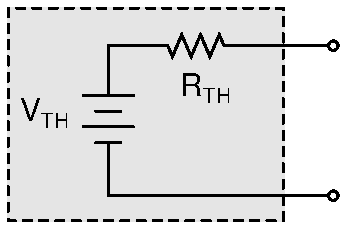
\includegraphics[width=0.55\textwidth]{./circuits/thevenin_circuit}
			\end{figure}
		\end{column}
		\begin{column}{.45\textwidth}
			\begin{block} {Norton's theorem}
				to a single current source
				$I_{N}$ and a single series resistor $R_{N}$ connected in parallel.
			\end{block}
			\begin{figure}
				\includegraphics[width=0.55\textwidth]{./circuits/norton_circuit}
			\end{figure}
		\end{column}
	\end{columns}

	\center Note above circuits are equivalent to each other when\\
	\center $R_{th} = R_N$ and $I_N = V_{th}/R_{th}$
\end{frame}

\begin{frame}
 \frametitle{Th\'evenin's and Norton's equivalent circuit example}
 \begin{block}{Problem}
  Determine the Th\'evenin equivalent circuit when:
  \begin{itemize}
   \item Open-circuit voltage is 2\,V
   \item Voltage drop for resistor of 1\,k$\Omega$ is 1\,V
  \end{itemize}
 \end{block}
 \begin{block}{Solution}
  \begin{itemize}
   \item Open-circuit voltage is $V_{th} = 2$\,V
   \item Resistor between terminals: unloaded voltage divider with $V = V_{th} \frac{R}{R_{th} + R}$, so $R_{th} = 1$\,k$\Omega$
  \end{itemize}
 \end{block}
\end{frame}


\begin{frame}
 \frametitle{Relevance of Th\'evenin and Norton Circuits}
 \begin{block}{Abstraction}
  \begin{itemize}
   \item Complicated circuits will consist of many 'sub-blocks' that we will want to simplify.
   \item Th\'evenin's theorem allows us to consider each sub-block as a single $V_{th}$ and $R_{th}$.
   \item Sub-blocks are characterized by open-circuit voltage and short-circuit current.
  \end{itemize}
 \end{block}
\end{frame}


\section{Voltage divider}
\begin{frame}
\frametitle{Voltage Divider}
\begin{columns}[t]
 \begin{column}{.45\textwidth}
  \begin{block}{Unloaded}
   \begin{figure}
    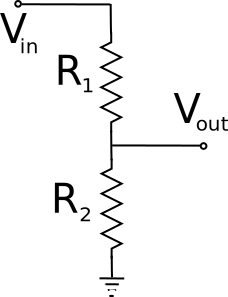
\includegraphics[height=1.5in]{./pics/unloaded_voltage_divider}
   \end{figure}
   \[ V_{out} = V_{in} \frac{R_2}{R_1+R_2} \]
  \end{block}
 \end{column}
  \begin{column}{.45\textwidth}
  \begin{block}{Loaded}
   \begin{figure}
    \includegraphics[height=1.5in]{./pics/loaded_voltage_divider}
   \end{figure}
   \[ V_{out} = V_{in} \frac{R_2}{R_1+R_2} \frac{R_L}{R_L + R_{1||2}} \]
   \[ V_{out} = V_{out,unloaded} \frac{R_L}{R_{1||2} + R_L} \]
  \end{block}
 \end{column}
\end{columns}
\end{frame}

\begin{frame}
 \frametitle{Voltage Divider: Power Dissipation}
 \begin{block}{Th\'evenin equivalent of unloaded voltage divider}
  Determine the Th\'evenin equivalent circuit:
  \begin{itemize}
   \item Open-circuit voltage is $V_{th} = V_{in} \frac{R_2}{R_1+R_2}$
   \item Short-circuit current is $I_{N} = \frac{V_{in}}{R_1} = \frac{V_{th}}{R_{th}}$
  \end{itemize}
  Th\'evenin resistance $R_{th} = \frac{V_{th}}{I_{N}} = R_{1||2}$
 \end{block}
 \begin{block}{Equivalent circuit of loaded voltage divider}
  Becomes very simple diagram with $V_{th}$ in series with $R_{th}$ and $R_{L}$
 \end{block}
\end{frame}

\begin{frame}
 \frametitle{Voltage Divider: Power Dissipation}
 \begin{block}{Power dissipation in loaded voltage divider}
  \begin{itemize}
   \item Current $I = \frac{V_{th}}{R_{th} + R_{L}}$
   \item Total power $P = R_{th} I^2 + R_{L} I^2 = \frac{V_{th}^2}{R_{th} + R_{L}}$
   \item Power in load $P_L = R_{L} I^2 = R_{L}  \frac{V_{th}^2}{(R_{th} + R_{L})^2}$
  \end{itemize}
 \end{block}
 Design exercise: for which $R_L$ is the power dissipated in the load maximal? (section 1.7)
 \\
 Hint:
 \begin{equation*}
  \frac{d P_L}{d R_L} = 0
 \end{equation*}
\end{frame}

\end{document}
